\documentclass[12pt, letterpaper]{article}

\usepackage{graphicx}
\usepackage{amsmath}

\title{Positron Emission Tomography}
\author{Jay Shen}
\date{April 2025}

\begin{document}

\maketitle

Positron emission tomography (PET) is a technique for imaging objects using radiation. In this lab, we make use of a simple PET setup to image a collection of radiation source distributions. 

\section{PET Apparatus}

\subsection{Motor Pulse Calibration}

Here, we make use of a PET apparatus composed of a rotary platform mounted on a linear track and a PMT coincidence detector. Before we use the setup, we must determine the conversion factors from motor pulses, with which we control the linear track, and the actual distance traveled by the platform. We took several measurements: each time we did a lateral reset, moved the platform by some number of pulses, and then measured the distance traveled. This data and a linear regression, from which we get conversion factors, are shown in Figure \ref{fig:calibration}. 
\begin{figure}
    \centering
    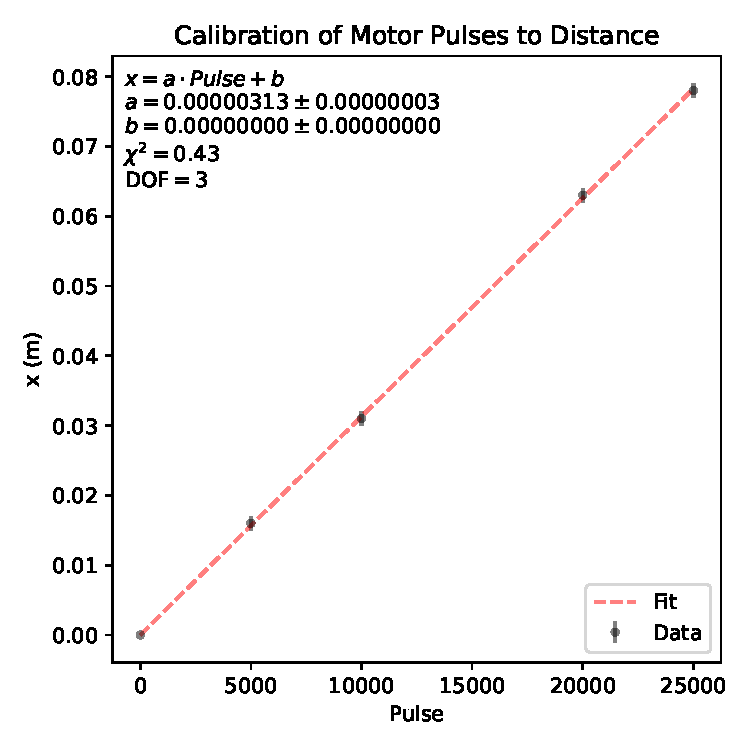
\includegraphics[width=0.5\linewidth]{experiment5/figures/calibration.pdf}
    \caption{Calibrating the lateral motor via linear regression achieves an excellent fit with minimal uncertainty.}
    \label{fig:calibration}
\end{figure}
From the fit, we get a conversion factor of $(3.13 \pm 0.03) \cdot 10^{-6}$ meters per pulse. The rotary pulse conversion factor was provided to be $\frac{180}{25600}$ degrees per pulse. We assume there is negligible uncertainty in this provided value. 

\subsection{1D PET of one source}\label{sec:resolution}

To test our setup, we place a single Na-22 source on the platform and executed a PET cycle. To determine both the location of the source on the platform, we choose to fit a mixture of two Gaussians to our data. One Gaussian conveniently models background noise while the other models the true peak produced by the source. From the peak Gaussian, we derive our metric for resolution: the full width at half maximum ($FWHM = 2 \sigma \sqrt{2 \ln 2}$). We perform this fitting procedure for three one-source setups and show the fits and $FWHM$ values in Figure \ref{fig:one_source}. 
\begin{figure}
    \centering
    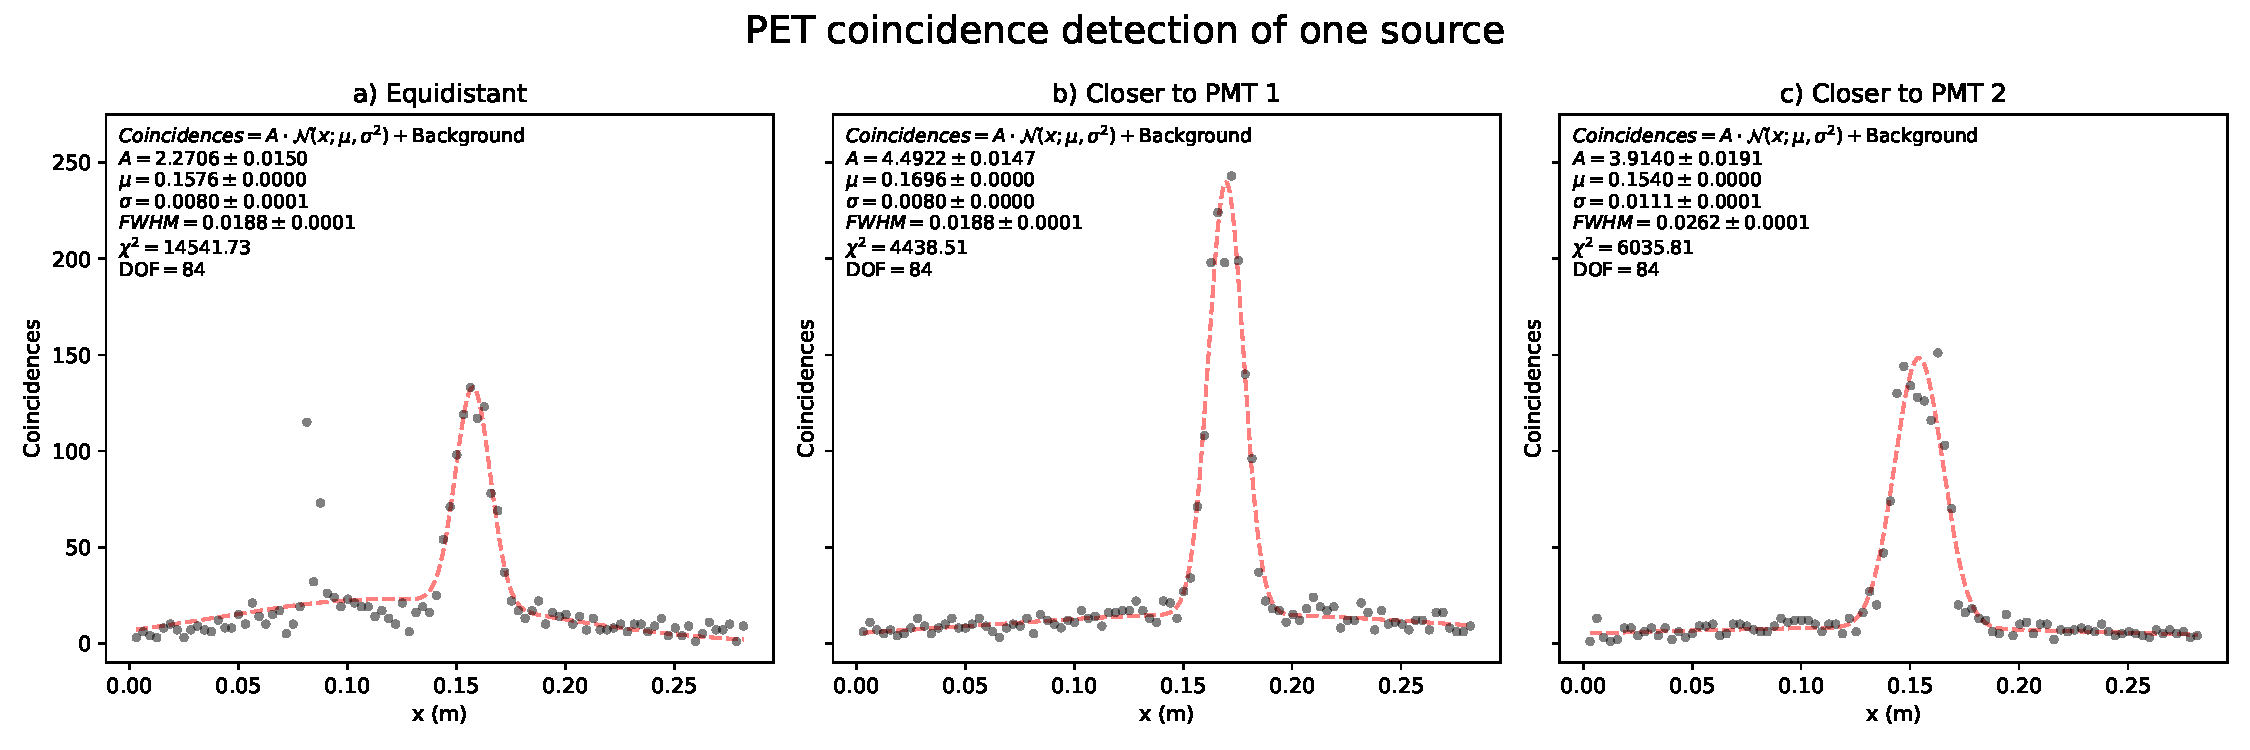
\includegraphics[width=1\linewidth]{experiment5/figures/one_source.pdf}
    \caption{1D PET data from a source that is a) equidistant from both PMTs, b) closer to PMT 1, and c) closer to PMT 2. As seen, the discrepancy between plots b) and c) indicate miscalibrated PMTs. }
    \label{fig:one_source}
\end{figure}

One conclusion from these trials is that our PMT setup is poorly calibrated, as otherwise Figures \ref{fig:one_source}b and \ref{fig:one_source}c should be the same. In lieu of a technical fix, we keep this in mind for the rest of the lab. Our second conclusion is that the resolution for one source is $W_1 = 0.0188 \pm 0.000122$ meters, which is the FWHM from Figure \ref{fig:one_source}a. 

\subsection{1D PET of two sources}

Now we take measurements for two source setups with varying amounts of separation. We wish to determine how close the sources can be before becoming indistinguishable from a single source. To quantify in-distinguishability, we again fit a sum of two Gaussians to the two-source data to model the noise and the peak(s). If the sources are indistinguishable, then the peak should resemble the single source peak and have a FWHM close to $W_1 = 0.0188 \pm 0.000122$. In the case of distinguishable sources, the FWHM will be larger than $W_1$. The data and fits for five different two-source setups are shown in \ref{fig:two_source}. 
\begin{figure}
    \centering
    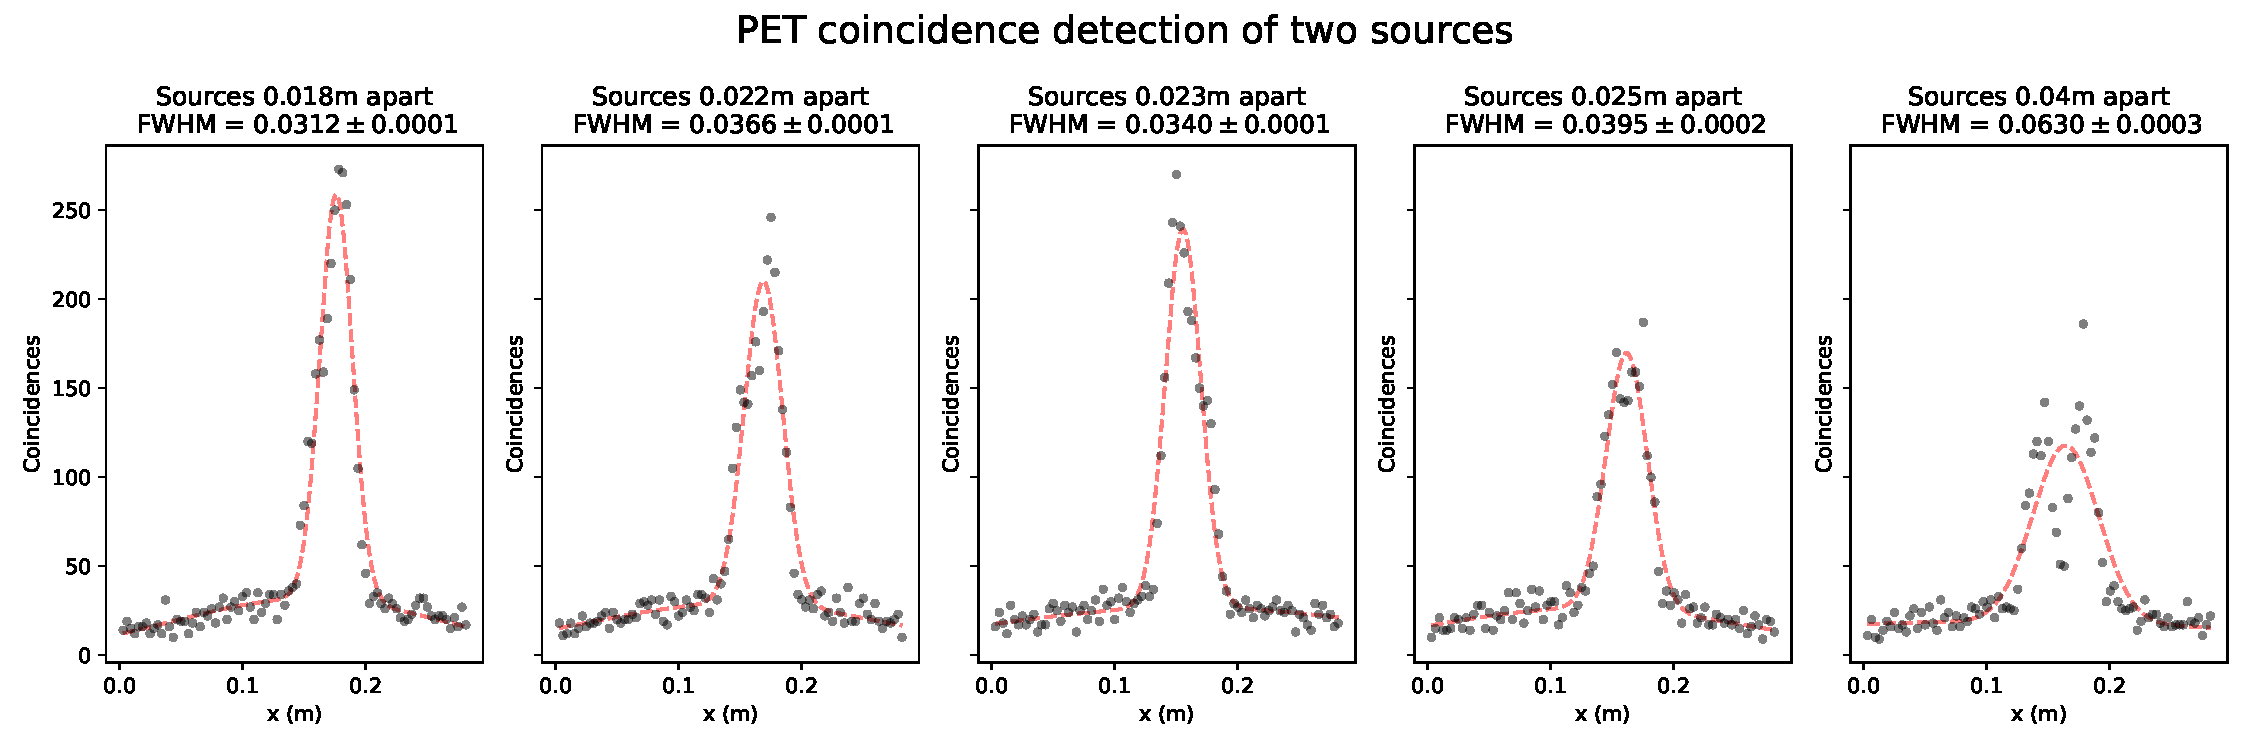
\includegraphics[width=1\linewidth]{experiment5/figures/two_sources.pdf}
    \caption{1D PET data taken of two sources at varying distances apart. }
    \label{fig:two_source}
\end{figure}

Unfortunately, as we see in from the plots, in all setups the sources are distinguishable by our metric. This is corroborated by a closer visual analysis, which reveals that all of the coincidence spreads are clearly bimodal, or exhibit shoulders, indicating the presence of two sources. At the time of data collection, we did not inspect our data carefully enough, and only upon post-hoc quantitative inspection did this problem reveal itself. 

However, we can still go ahead and estimate the distance of unresolvability. We fit a linear curve relating separation distance and FWHM in Figure \ref{fig:separation}. 
\begin{figure}
    \centering
    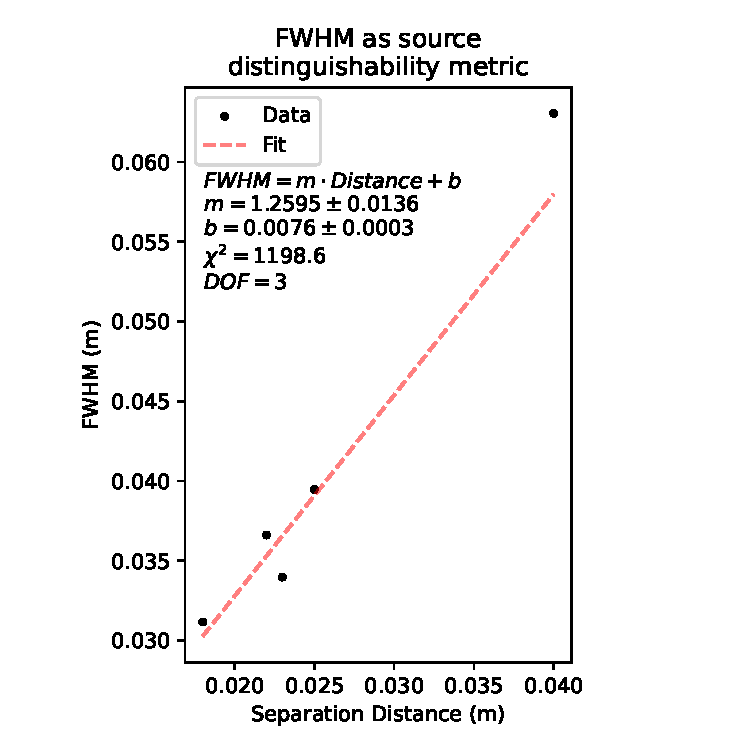
\includegraphics[width=0.5\linewidth]{experiment5/figures/separation.pdf}
    \caption{A linear regression predicting FWHM from separation distance. }
    \label{fig:separation}
\end{figure}
We extrapolate this curve to solve for where the FWHM equals $W_1 = 0.0188 \pm 0.000122$ and obtain $0.00893 \pm 0.000273$ meters as the minimum resolvable separation. 

\section{PET Imaging of Unknown Distribution}\label{sec:unknown}

Now we test our procedure on an unknown source distribution. We opt to traverse the linear track 40 times, each traversal taking 90 steps of 1000 pulses (around 3 milimeters) to cover the entire track. At each step, the PMTs scan for 20 seconds to obtain the best possible data within a reasonable time frame. At the end of each full traversal, the platform rotates 320 pulses, or 4.5 degrees. That way, we achieve a full 180 degree rotation. The sinogram relating angle, lateral position, and number of coincidences is shown in Figure \ref{fig:unknown_sinogram}. 
\begin{figure}
    \centering
    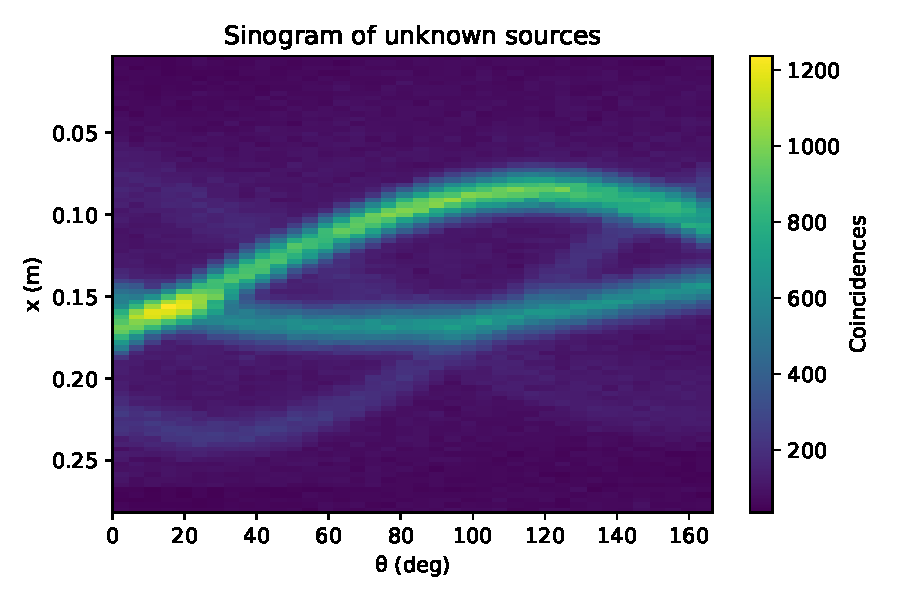
\includegraphics[width=0.75\linewidth]{experiment5/figures/unknown_sinogram.pdf}
    \caption{Sinogram from PET loop of unknown sources. }
    \label{fig:unknown_sinogram}
\end{figure}
An inverse Radon transform is applied to the sinogram to reconstruct the source distribution, as shown in Figure \ref{fig:unknown_reconstruction}. 

\begin{figure}
    \centering
    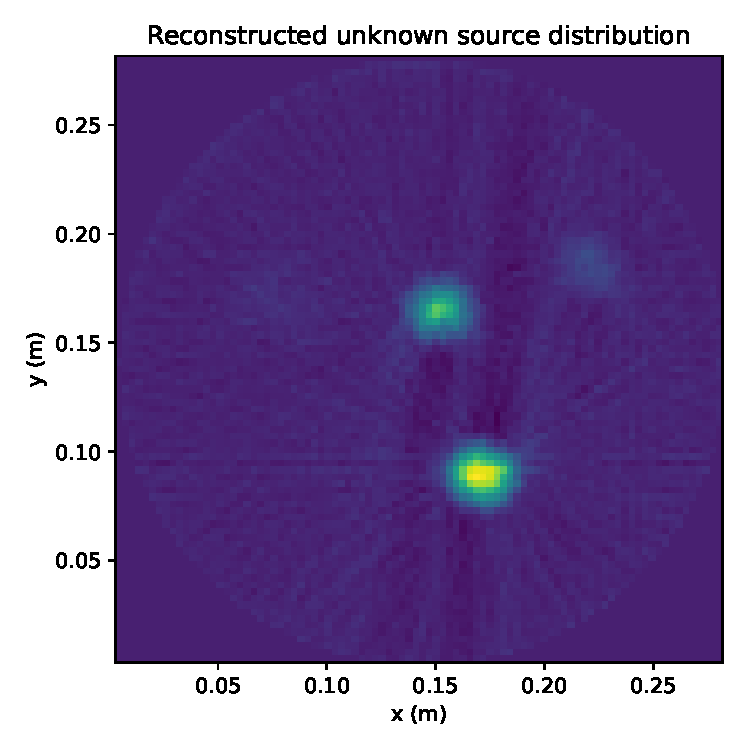
\includegraphics[width=0.75\linewidth]{experiment5/figures/unknown_reconstruction.pdf}
    \caption{Reconstruction of unknown source distribution using inverse Radon transform of PET sinogram. }
    \label{fig:unknown_reconstruction}
\end{figure}

To determine the positions of the sources, we identify a source peak by hand, then fit a 2D isotropic Gaussian function to it. The mean of the fitted peak corresponds to the source position estimate, and its amplitude corresponds to the source intensity. Uncertainty is automatically computed through the fitting software. The fitting process is shown in Figure \ref{fig:unknown_fitting} and the extracted source coordinates are shown in Figure \ref{fig:unknown_positions} and listed in Table \ref{tab:unknown_positions}. 

\begin{figure}
    \centering
    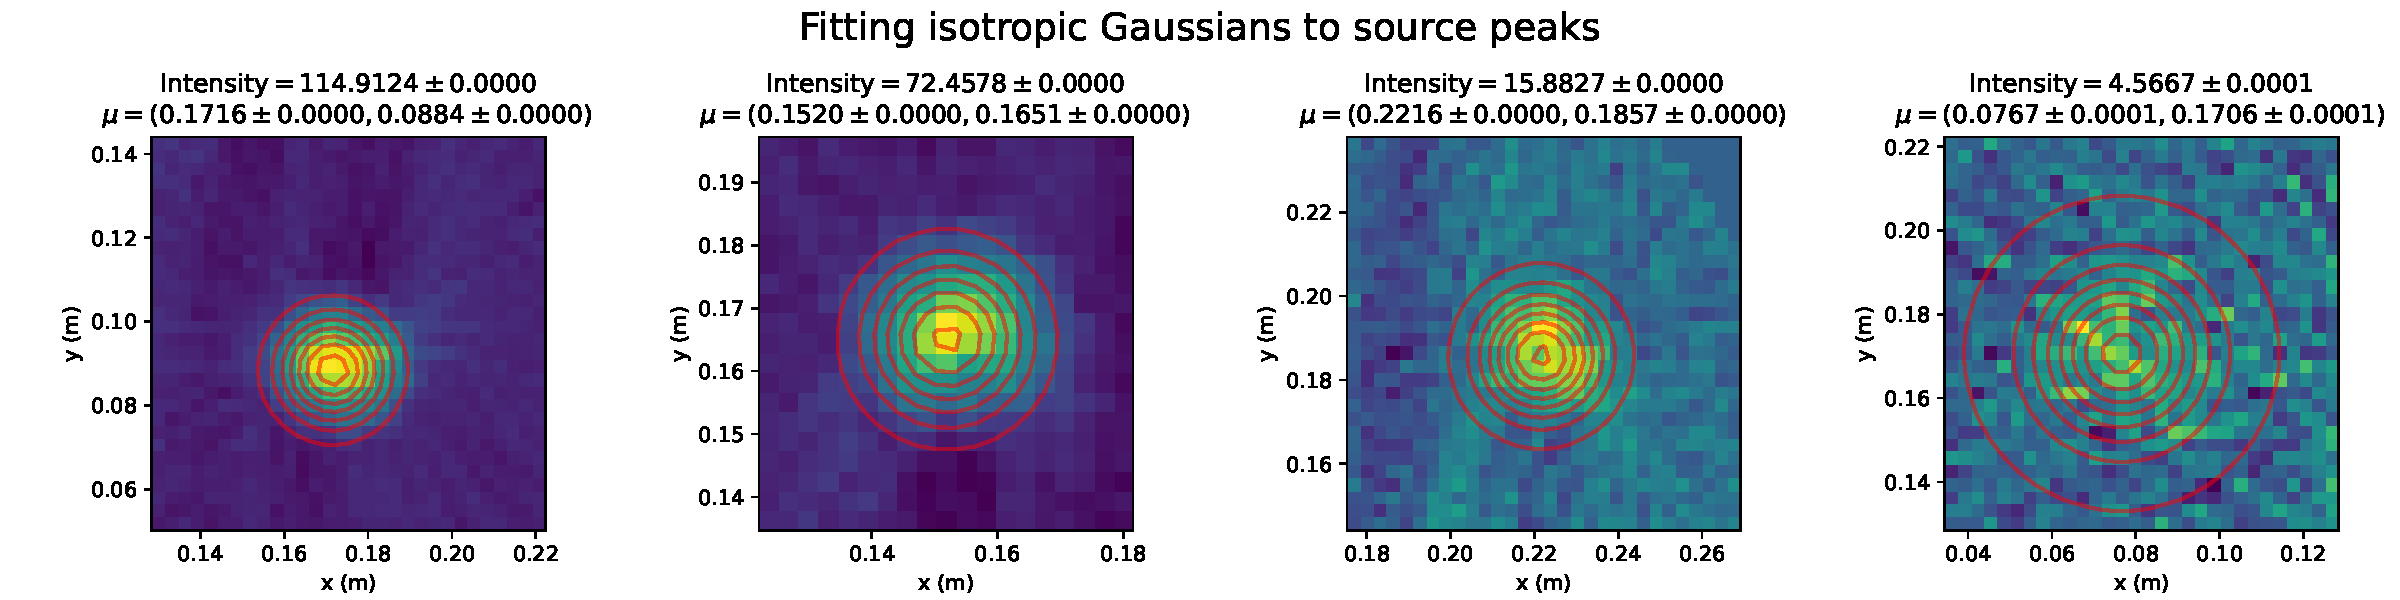
\includegraphics[width=1\linewidth]{experiment5/figures/unknown_fitting.pdf}
    \caption{Fitting 2D Gaussians enables principled identification of source positions. }
    \label{fig:unknown_fitting}
\end{figure}

\begin{figure}
    \centering
    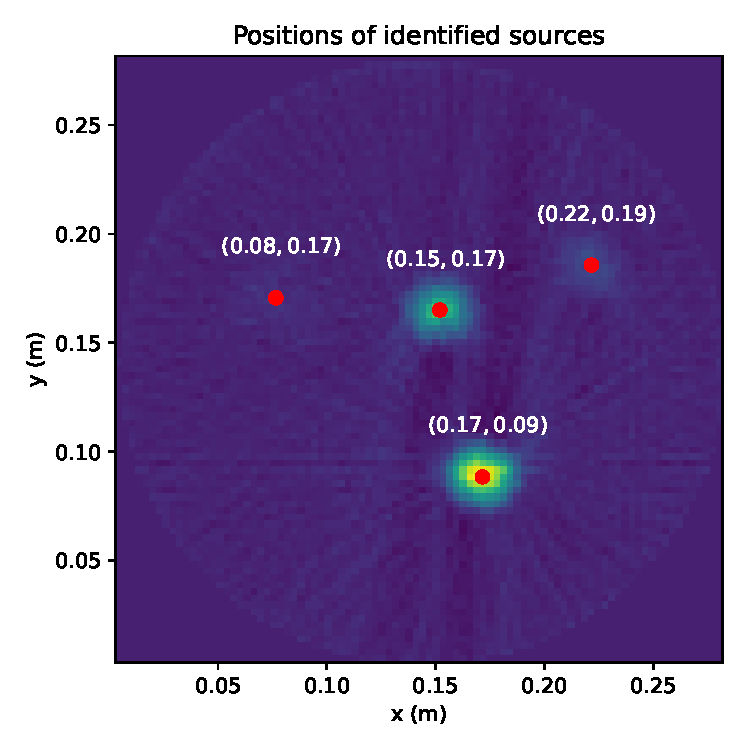
\includegraphics[width=0.75\linewidth]{experiment5/figures/unknown_positions.pdf}
    \caption{Final positions identified using PET procedure. }
    \label{fig:unknown_positions}
\end{figure}

\begin{table}[]
    \centering
    \begin{tabular}{| c | c | c |}
        \hline
        x (m) & y (m) & Intensity ($\frac{\text{coincidences}}{9.8 \cdot 10^{-6} \text{ m}^2}$) \\
        \hline
        $0.171570 \pm 0.000002$ & $0.088443 \pm 0.000002$ & $114.912353 \pm 0.028583$ \\
        $0.152015 \pm 0.000003$ & $0.165061 \pm 0.000003$ & $72.457780 \pm 0.028878$ \\
        $0.221620 \pm 0.000016$ & $0.185696 \pm 0.000016$ & $15.882722 \pm 0.025075$ \\
        $0.076663 \pm 0.000055$ & $0.170644 \pm 0.000055$ & $4.566706 \pm 0.018906$ \\
        \hline
    \end{tabular}
    \caption{Positions and intensities for identified sources. }
    \label{tab:unknown_positions}
\end{table}

\section{PET Imaging of Challenge Distribution}

To image an unknown distribution under time constraints, we elect to change the values of all tomography variables. We complete 8 iterations of a full lateral sweep, taking 45 steps of 2000 lateral motor pulses (around 6.3 millimeters). At each step we scan for 5 seconds. At the end of each iteration, we rotate by 1600 rotary motor pulses (around 22.5 degrees), to capture the full 180 degrees. We chose these parameters heuristically under the assumption that all degrees of freedom are equally important and that we should not prioritize one or the other. The sinogram and reconstruction are shown in Figures \ref{fig:challenge_sinogram} and \ref{fig:challenge_reconstruction}. 
\begin{figure}
    \centering
    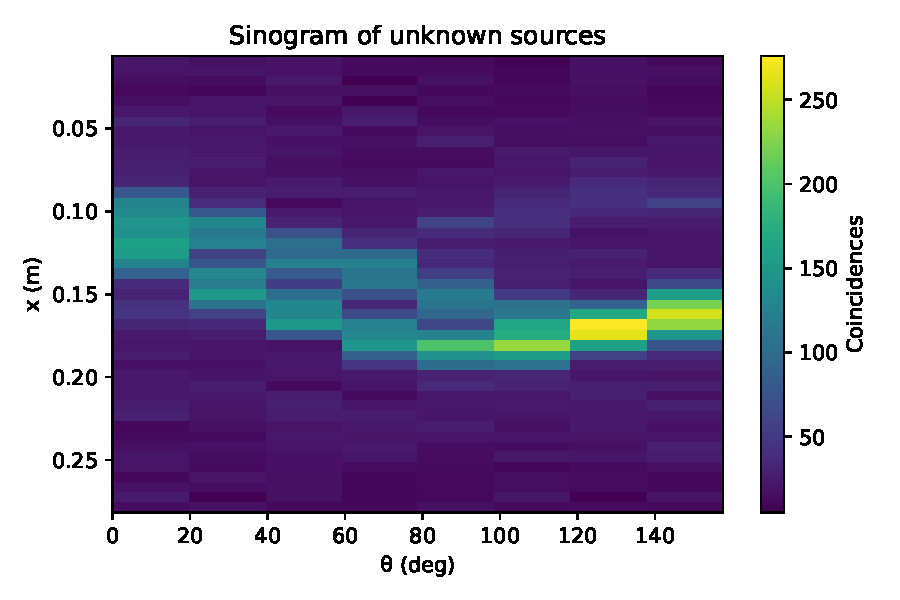
\includegraphics[width=0.75\linewidth]{experiment5/figures/challenge_sinogram.pdf}
    \caption{Sinogram for unknown challenge distribution. }
    \label{fig:challenge_sinogram}
\end{figure}
\begin{figure}
    \centering
    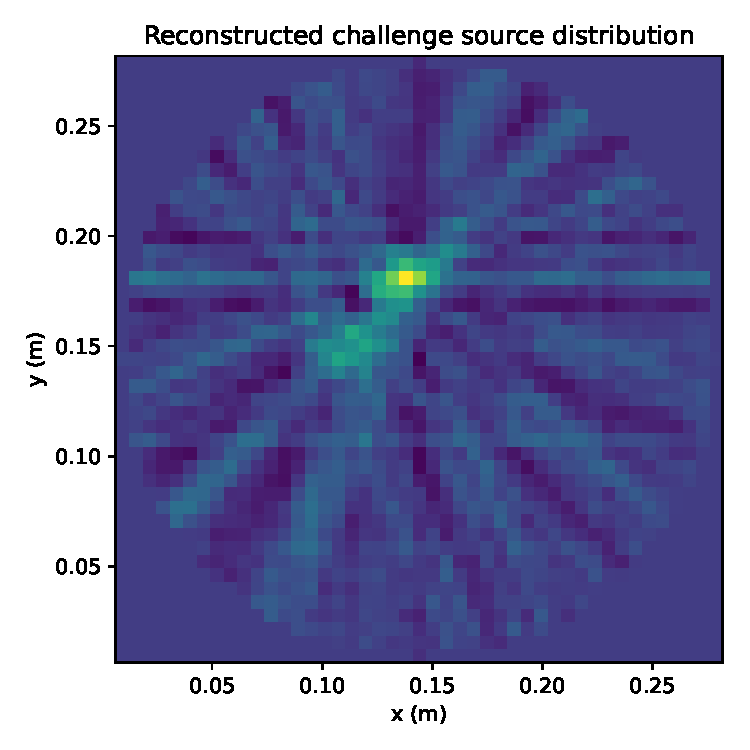
\includegraphics[width=0.75\linewidth]{experiment5/figures/challenge_reconstruction.pdf}
    \caption{Reconstruction of unknown challenge distribution. }
    \label{fig:challenge_reconstruction}
\end{figure}
We follow the same procedure from Section \ref{sec:unknown} to determine the position of the most intense source. The fitted Gaussian contour is shown in Figure \ref{fig:challenge_fitting}. 

\begin{figure}
    \centering
    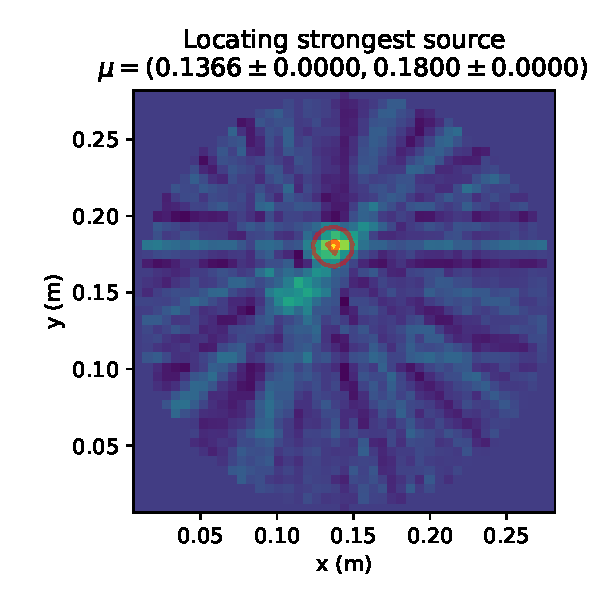
\includegraphics[width=0.75\linewidth]{experiment5/figures/challenge_fitting.pdf}
    \caption{Fitting a 2D Gaussian to the strongest identified source. We identify the location of the strongest source to be $(0.136604 \pm 0.000015, 0.180013 \pm 0.000015)$}
    \label{fig:challenge_fitting}
\end{figure}

In such a way, we are able to identify the source location within a negligible margin of error and with limited time. Whether or not the location we found is accurate remains to be seen. However, we hypothesize that our method is actually not suited to coarse data such as this. This is because fitting the Gaussian inevitably takes into account all the smears and imperfections, achieving a biased fit. We also hypothesize that taking measurements for more values of $\theta$, and letting the lateral resolution be coarser, will achieve better results. This is evidenced by the streaky appearance of the reconstruction, the redundancy of some lateral positions, and the ways our fitting software struggled. 

\section{Conclusion}

To conclude, we observed the use of a PET setup for imaging distributions of positron sources. We evaluated one approach to determining positions within PET reconstructions, and also identified critical parts of the procedure to refine in the future. 

\end{document}
